% ============================================================
%  RoadFury -- ICST 2026 SDC Tool Competition
%  Conference presentation slides  (~10 min talk)
%  Compile: pdflatex roadfury_icst2026.tex  (twice for refs)
% ============================================================
\documentclass[aspectratio=169,10pt]{beamer}

\usetheme{metropolis}
\usecolortheme{metropolis}
\usefonttheme{professionalfonts}
\setbeamertemplate{frame numbering}[fraction]
\setbeamertemplate{itemize item}{\textcolor{mLightBrown}{\scriptsize$\blacktriangleright$}}
\setbeamertemplate{itemize subitem}{\textbullet}
\setbeamertemplate{itemize subsubitem}{--}

% ---- Packages ----
\usepackage{amsmath, amssymb}
\usepackage[utf8]{inputenc}
\usepackage[T1]{fontenc}
\usepackage[english]{babel}
\usepackage{booktabs}
\usepackage[table]{xcolor}
\usepackage{tikz}
\usepackage{pgfplots}
\usepackage{array}
\usepackage{graphicx}
\usepackage{adjustbox}
\usepackage{hyperref}
\usepackage{colortbl}
\pgfplotsset{compat=1.18}
\usetikzlibrary{shapes.geometric, arrows.meta, positioning, calc, fit, backgrounds}

% ---- Palette ----
\definecolor{mDarkTeal}{HTML}{23373B}
\definecolor{mLightBrown}{HTML}{EB811B}
\definecolor{softgray}{HTML}{F2F4F7}
\definecolor{tealtint}{HTML}{D6DEE0}
\definecolor{successgreen}{HTML}{1A7A3C}
\definecolor{alertred}{HTML}{C0392B}
\definecolor{teallight}{HTML}{2E8B8F}

\colorlet{accent}{mLightBrown}
\colorlet{success}{successgreen}
\colorlet{alert}{alertred}

\hypersetup{colorlinks=true, urlcolor=mLightBrown, linkcolor=mDarkTeal}
\renewcommand{\arraystretch}{1.2}

% Convenience: highlight a number
\newcommand{\hl}[1]{\textcolor{mLightBrown}{\textbf{#1}}}
\newcommand{\hlg}[1]{\textcolor{successgreen}{\textbf{#1}}}
\newcommand{\hlr}[1]{\textcolor{alertred}{\textbf{#1}}}

% ============================================================
%  TITLE / META
% ============================================================
\title[RoadFury @ ICST 2026]{%
  \textbf{RoadFury}: Transformer-Based Test Prioritization\\
  for Self-Driving Cars}
\subtitle{ICST 2026 Tool Competition -- SDC Testing Track}
\author[Tran et al.]{%
  Chi-Nguyen Tran$^*$\quad
  Dao Sy Duy Minh$^*$\quad
  Huynh Trung Kiet$^*$\\[3pt]
  Phu-Hoa Pham\quad
  Nguyen Lam Phu Quy\\[4pt]
  {\small\itshape $^*$Equal contribution}
}
\institute{%
  Faculty of Information Technology\\
  University of Science (HCMUS), VNU-HCM, Vietnam
}
\date{ICST 2026}

% ============================================================
\begin{document}
% ============================================================

%% ---- Title slide ----
\begin{frame}[plain]
  \titlepage
\end{frame}

%% ---- Outline ----
\begin{frame}{Talk Outline}
  \setbeamertemplate{section in toc}[sections numbered]
  \tableofcontents[hideallsubsections]
\end{frame}

% ============================================================
\section{Motivation \& Problem}
% ============================================================

\begin{frame}{SDC Testing is Expensive}
  \begin{columns}[T]
    \begin{column}{0.55\linewidth}
      \begin{itemize}
        \item Simulators (BeamNG.tech) enable large-scale testing
        \item Each simulation run takes \textbf{minutes} of wall-clock time
        \item A full test suite may contain \textbf{thousands} of road scenarios
        \item Goal: \emph{run failing tests first} -- maximize early fault detection
      \end{itemize}
      \vspace{6pt}
      \begin{block}{APFD -- the standard metric}
        \[
          \text{APFD}(\pi)=1-\frac{\sum_{i=1}^{m}TF_i}{n\cdot m}+\frac{1}{2n}
        \]
        Higher APFD $\Rightarrow$ faults exposed earlier.\\
        Random baseline $\approx 0.50$.
      \end{block}
    \end{column}
    \begin{column}{0.42\linewidth}
      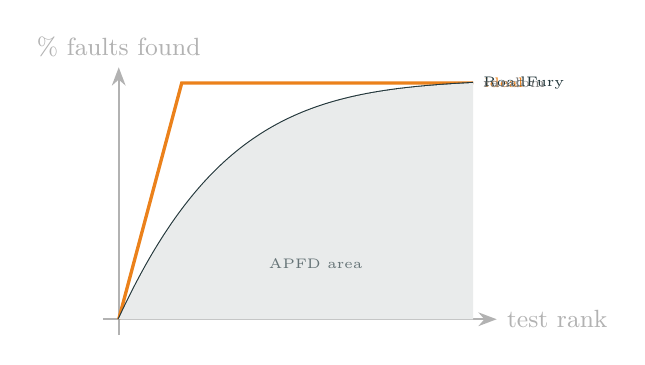
\begin{tikzpicture}[font=\small, >=Stealth]
        \draw[thick, ->, gray!60] (-0.2,0) -- (4.8,0) node[right] {test rank};
        \draw[thick, ->, gray!60] (0,-0.2) -- (0,3.2) node[above] {\% faults found};
        % ideal
        \draw[mLightBrown, very thick] (0,0) -- (0.8,3.0) -- (4.5,3.0)
              node[right, font=\tiny] {ideal};
        % RoadFury (high APFD)
        \draw[mDarkTeal, thick] (0,0) .. controls (1.2,2.6) and (2.5,2.9) .. (4.5,3.0)
              node[right, font=\tiny, text=mDarkTeal] {RoadFury};
        % random
        \draw[gray, dashed] (0,0) -- (4.5,3.0) node[right, font=\tiny, gray] {random};
        % shaded area
        \fill[mDarkTeal!10] (0,0) .. controls (1.2,2.6) and (2.5,2.9) .. (4.5,3.0)
          -- (4.5,0) -- cycle;
        \node[font=\tiny, mDarkTeal!70] at (2.5,0.7) {APFD area};
      \end{tikzpicture}
    \end{column}
  \end{columns}
\end{frame}

\begin{frame}{The Gap: Aggregate Statistics vs.\ Full Geometry}
  \begin{columns}[T]
    \begin{column}{0.48\linewidth}
      \textbf{\hlr{Existing tools (e.g., SDC-Scissor)}}
      \vspace{4pt}
      \begin{itemize}
        \item Summarize each road by 3 scalars:\\
              mean curvature, lateral pos., std
        \item Feed into a feedforward network
        \item Discards \emph{spatial transitions}:\\
              consecutive sharp bends, jerk spikes
      \end{itemize}
      \vspace{10pt}
      {\small APFD$_\text{best prior}$ = 0.781 (ITEP4SDC)}
    \end{column}
    \begin{column}{0.48\linewidth}
      \textbf{\hlg{RoadFury insight}}
      \vspace{4pt}
      \begin{itemize}
        \item Road = \emph{ordered sequence} of geometry
        \item Preserve all 197 points
        \item 10 intrinsic channels per point\\
              (curvature, jerk, heading, \ldots)
        \item Transformer attends over the full trajectory
      \end{itemize}
      \vspace{10pt}
      {\small \hlg{APFD = 0.804 $\pm$ 0.012} -- new best}
    \end{column}
  \end{columns}
\end{frame}

% ============================================================
\section{Approach}
% ============================================================

\begin{frame}{Step 1 -- Road Geometry Feature Extraction}
  \begin{columns}[T]
    \begin{column}{0.50\linewidth}
      \begin{enumerate}
        \item Uniformly resample road to $L{=}197$ points
        \item Compute \textbf{10 intrinsic geometry channels} at each point
        \item Z-normalize per channel (training set stats)
        \item Result: $(197{\times}10)$ feature matrix -- \textbf{translation- \& rotation-invariant}
      \end{enumerate}
    \end{column}
    \begin{column}{0.47\linewidth}
      \small
      \begin{tabular}{@{}clp{2.3cm}@{}}
        \toprule
        \textbf{Ch.} & \textbf{Feature} & \textbf{Captures} \\
        \midrule
        $f_0$ & Seg.\ length    & road scale \\
        $f_1$ & Abs.\ angle     & local bend \\
        $f_2$ & Menger curv.    & sharpness \\
        $f_3$ & Curv.\ jerk     & \hl{sudden changes} \\
        $f_4$ & Cum.\ dist.     & arc progress \\
        $f_5,f_6$ & $\sin/\cos\theta$ & heading \\
        $f_7$ & Rel.\ pos.      & position in road \\
        $f_8$ & Local curv.\ std & \hl{cluster of bends} \\
        $f_9$ & Curv.\ accel.   & 2nd-order dynamics \\
        \bottomrule
      \end{tabular}
    \end{column}
  \end{columns}
\end{frame}

\begin{frame}{Step 2 -- RoadTransformer Architecture}
  \begin{center}
  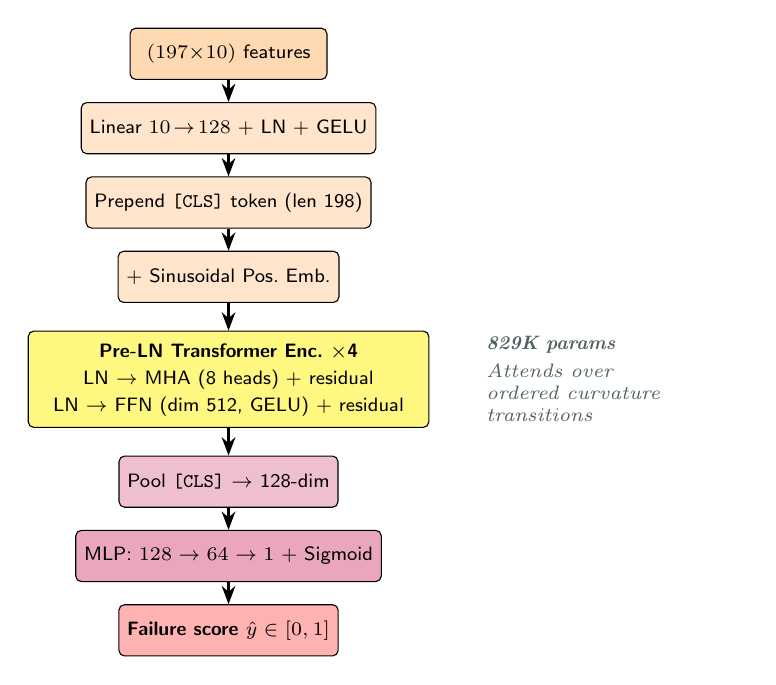
\begin{tikzpicture}[
    font=\sffamily\scriptsize, >=Stealth,
    node distance=0.28cm,
    blk/.style={draw, rounded corners=2pt, fill=#1, align=center,
                inner sep=3pt, minimum width=2.5cm, minimum height=0.65cm},
  ]
    % Left column: feature
    \node[blk=orange!30] (inp) {$(197{\times}10)$ features};
    \node[blk=orange!20, below=of inp] (proj) {Linear $10\!\to\!128$ + LN + GELU};
    \node[blk=orange!20, below=of proj] (cls) {Prepend \texttt{[CLS]} token (len 198)};
    \node[blk=orange!20, below=of cls] (pos) {+ Sinusoidal Pos.\ Emb.};

    % Transformer block
    \node[blk=yellow!50, minimum height=1.1cm, below=0.35cm of pos] (enc) {%
      \begin{tabular}{c}
        \textbf{Pre-LN Transformer Enc.\ $\times$4}\\
        LN $\to$ MHA (8 heads) + residual\\
        LN $\to$ FFN (dim 512, GELU) + residual
      \end{tabular}};

    % Right column
    \node[blk=purple!25, below=0.35cm of enc] (pool) {Pool \texttt{[CLS]} $\to$ 128-dim};
    \node[blk=purple!35, below=of pool] (mlp)  {MLP: $128\to64\to1$ + Sigmoid};
    \node[blk=red!30, below=of mlp] (out) {\textbf{Failure score $\hat{y}\in[0,1]$}};

    \draw[->, thick] (inp) -- (proj);
    \draw[->, thick] (proj) -- (cls);
    \draw[->, thick] (cls) -- (pos);
    \draw[->, thick] (pos) -- (enc);
    \draw[->, thick] (enc) -- (pool);
    \draw[->, thick] (pool) -- (mlp);
    \draw[->, thick] (mlp) -- (out);

    % annotation
    \node[right=0.6cm of enc, text width=3.2cm, font=\scriptsize\itshape, text=mDarkTeal!80] {
      \textbf{829K params}\\[2pt]
      Attends over\\
      ordered curvature\\
      transitions
    };
  \end{tikzpicture}
  \end{center}
\end{frame}

\begin{frame}{Step 3 -- Stochastic Weight Averaging (SWA)}
  \begin{columns}[T]
    \begin{column}{0.55\linewidth}
      \textbf{Training recipe:}
      \begin{itemize}
        \item Dataset: \textbf{28,804} labeled road-outcome pairs (SensoDat)
        \item Optimizer: AdamW, lr$=5{\times}10^{-4}$, 75 epochs
        \item Loss: Binary Cross-Entropy
        \item SWA: average checkpoints from epochs 50--75
      \end{itemize}
      \vspace{8pt}
      \textbf{Why SWA?}
      \begin{itemize}
        \item Finds \emph{flatter} loss landscape minima
        \item Translates to better generalization on unseen roads
        \item +\,0.016 APFD over no-SWA (ablation confirms)
      \end{itemize}
    \end{column}
    \begin{column}{0.42\linewidth}
      \begin{center}
      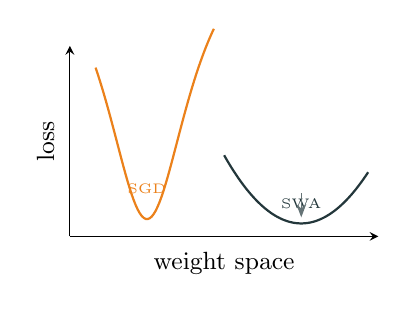
\begin{tikzpicture}[font=\small, >=Stealth]
        \begin{axis}[
          width=5.5cm, height=4cm,
          xlabel={weight space}, ylabel={loss},
          xtick=\empty, ytick=\empty,
          axis lines=left,
          ymin=0, ymax=2.2,
          xmin=0, xmax=6,
          clip=false,
        ]
          % sharp minimum (SGD)
          \addplot[mLightBrown, thick, domain=0.5:2.8, samples=60]
            {0.2 + 3.5*(x-1.5)^2 / (1 + (x-1.5)^2)};
          % flat minimum (SWA)
          \addplot[mDarkTeal, thick, domain=3.0:5.8, samples=60]
            {0.15 + 0.35*(x-4.5)^2};
          \node[mLightBrown, font=\tiny] at (axis cs:1.5,0.55) {SGD};
          \node[mDarkTeal, font=\tiny] at (axis cs:4.5,0.38) {SWA};
          \draw[->, thin, mDarkTeal!70] (axis cs:4.5,0.5) -- (axis cs:4.5,0.22);
        \end{axis}
      \end{tikzpicture}
      \end{center}
      \vspace{-4pt}
      {\small\itshape SWA finds flatter optima $\Rightarrow$ better generalization}
    \end{column}
  \end{columns}
\end{frame}

\begin{frame}{Step 4 -- Deployment as gRPC Microservice}
  \begin{columns}[T]
    \begin{column}{0.52\linewidth}
      \textbf{Docker-containerized gRPC service:}
      \vspace{4pt}
      \begin{enumerate}
        \item Receive batch of test cases (road points) via gRPC
        \item Compute $(n, 197, 10)$ feature tensor
        \item Forward pass through RoadTransformer
        \item Score each road $\Rightarrow$ sort descending by $\hat{y}$
        \item Return \textbf{prioritized test IDs}
      \end{enumerate}
      \vspace{8pt}
      \textbf{Three endpoints:}\\
      \texttt{Name} \quad \texttt{Initialize} \quad \texttt{Prioritize}
    \end{column}
    \begin{column}{0.44\linewidth}
      \begin{block}{Integration with competition platform}
        \begin{itemize}
          \item Plug-and-play Docker container
          \item Competition framework calls \texttt{Prioritize}
          \item Returns ranked list in $<$1\,s for 956 tests
        \end{itemize}
      \end{block}
      \vspace{6pt}
      \begin{alertblock}{Open-source}
        \url{github.com/chisngyen/\\sdc-test-prioritization-novel}
      \end{alertblock}
    \end{column}
  \end{columns}
\end{frame}

% ============================================================
\section{Results}
% ============================================================

\begin{frame}{Multi-Paradigm Comparison}
  \textbf{956-test competition set, 30 independent random trials}
  \vspace{6pt}

  \begin{center}
  \begin{tabular}{lcc}
    \toprule
    \textbf{Method} & \textbf{APFD} & \textbf{Paradigm} \\
    \midrule
    Random                   & 0.493              & -- \\
    LLM zero-shot            & 0.487\,$\pm$\,0.019 & Language model \\
    GNN (road graph)         & 0.533\,$\pm$\,0.025 & 3-layer GCN \\
    ResNet-50 visual         & 0.572\,$\pm$\,0.013 & Road image CNN \\
    ITEP4SDC (prior best)    & 0.781              & MLP, 3 features \\
    \rowcolor{mLightBrown!20}
    \textbf{RoadFury (ours)} & \textbf{0.804\,$\pm$\,0.012} & \textbf{Transformer+SWA} \\
    \bottomrule
  \end{tabular}
  \end{center}

  \vspace{6pt}
  \begin{columns}[T]
    \begin{column}{0.30\linewidth}
      \begin{block}{\small vs.\ random}
        \centering +63\% relative gain
      \end{block}
    \end{column}
    \begin{column}{0.30\linewidth}
      \begin{block}{\small vs.\ best prior}
        \centering +0.023 APFD absolute
      \end{block}
    \end{column}
    \begin{column}{0.35\linewidth}
      \begin{alertblock}{\small Key}
        Sequence matters:\\LLM, GNN, CNN all miss it
      \end{alertblock}
    \end{column}
  \end{columns}
\end{frame}

\begin{frame}{Why Not LLM / GNN / CNN?}
  \begin{columns}[T]
    \begin{column}{0.30\linewidth}
      \textbf{\hlr{LLM zero-shot}}\\[4pt]
      0.487 $\pm$ 0.019 (worse than random)
      \vspace{6pt}
      \begin{itemize}
        \item Reasons over text descriptions
        \item Misses fine-grained numeric geometry
        \item No ordered curvature signal
      \end{itemize}
    \end{column}
    \begin{column}{0.30\linewidth}
      \textbf{\hlr{GNN}}\\[4pt]
      0.533 $\pm$ 0.025
      \vspace{6pt}
      \begin{itemize}
        \item Captures pairwise adjacency
        \item Loses \emph{ordered} trajectory dynamics
        \item Permutation-invariant by design
      \end{itemize}
    \end{column}
    \begin{column}{0.30\linewidth}
      \textbf{\hlr{ResNet CNN}}\\[4pt]
      0.572 $\pm$ 0.013
      \vspace{6pt}
      \begin{itemize}
        \item Renders road as image
        \item Sacrifices numeric precision of curvature
        \item Spatial pooling discards jerk
      \end{itemize}
    \end{column}
  \end{columns}
  \vspace{10pt}
  \begin{center}
  \large
  \hlg{Transformer over ordered curvature sequence wins because it preserves what matters.}
  \end{center}
\end{frame}

\begin{frame}{Ablation Study -- Only SWA Helps}
  \textbf{Base: RoadTransformer without SWA} (APFD = 0.788 $\pm$ 0.014)
  \vspace{6pt}

  \begin{center}
  \begin{tabular}{lc}
    \toprule
    \textbf{Modification} & \textbf{APFD} \\
    \midrule
    + Multi-scale Conv Stem       & \hlr{0.767 $\pm$ 0.014 $\downarrow$} \\
    + Stochastic Depth (DropPath) & \hlr{0.768 $\pm$ 0.015 $\downarrow$} \\
    + Triple Pooling (CLS+Mean+Max)& \hlr{0.768 $\pm$ 0.015 $\downarrow$} \\
    + Mixup augmentation          & \hlr{0.773 $\pm$ 0.015 $\downarrow$} \\
    + Focal Loss ($\gamma{=}2$)   & \hlr{0.782 $\pm$ 0.014 $\downarrow$} \\
    + Test-time augmentation (TTA)& \hlr{0.770 $\pm$ 0.016 $\downarrow$} \\
    \rowcolor{mLightBrown!20}
    \textbf{+ SWA}                & \hlg{\textbf{0.804 $\pm$ 0.012 $\uparrow$}} \\
    \bottomrule
  \end{tabular}
  \end{center}

  \vspace{4pt}
  {\small \textit{The recipe is simple: Pre-LN Transformer + SWA. Nothing else helps.}}
\end{frame}

% ============================================================
\section{Conclusion}
% ============================================================

\begin{frame}{Conclusion}
  \begin{columns}[T]
    \begin{column}{0.55\linewidth}
      \textbf{Key takeaways:}
      \begin{enumerate}
        \item \textbf{Sequential geometry matters}:\\
              aggregate statistics discard the spatial transitions that predict failures
        \item \textbf{Simple recipe wins}:\\
              Pre-LN Transformer + SWA, identical hyperparams
        \item \textbf{APFD = 0.804 $\pm$ 0.012}:\\
              new best in ICST 2026 SDC Competition\\
              ($+$0.023 over prior best ITEP4SDC)
        \item \textbf{Ablation confirms}: SWA is the single most impactful component
      \end{enumerate}
    \end{column}
    \begin{column}{0.42\linewidth}
      \begin{block}{Future Work}
        \begin{itemize}
          \item Richer simulation feedback signals (speed, steering torque)
          \item Cross-simulator transfer (BeamNG $\to$ CARLA)
          \item Theory-driven invariance probes (rotation, resolution)
          \item Conformal prediction bounds on APFD
        \end{itemize}
      \end{block}
      \vspace{6pt}
      \begin{alertblock}{Code \& data}
        \url{github.com/chisngyen/sdc-test-prioritization-novel}
      \end{alertblock}
    \end{column}
  \end{columns}
\end{frame}

%% ---- Q&A / Thank you ----
\begin{frame}[plain]
  \begin{center}
    \vspace{1.5cm}
    {\Large \textbf{Thank You!}}\\[12pt]
    {\large Questions?}\\[20pt]
    \hrule
    \vspace{10pt}
    {\small
    Chi-Nguyen Tran, Dao Sy Duy Minh, Huynh Trung Kiet,\\
    Phu-Hoa Pham, Nguyen Lam Phu Quy\\[4pt]
    \textit{University of Science (HCMUS), VNU-HCM}\\[6pt]
    \url{github.com/chisngyen/sdc-test-prioritization-novel}
    }
  \end{center}
\end{frame}

%% ---- Backup: Full Architecture Figure (optional) ----
\appendix

\begin{frame}[allowframebreaks]{Backup -- Architecture Details}
  \textbf{Model specification:}
  \vspace{4pt}
  \begin{itemize}
    \item Input: $(197{\times}10)$ z-normalized feature matrix
    \item Embedding: Linear $10\to128$ + LayerNorm + GELU
    \item Sequence: 198 tokens (197 road points + 1 CLS)
    \item Positional encoding: sinusoidal (fixed)
    \item Encoder: 4$\times$ Pre-LN Transformer layers
      \begin{itemize}
        \item Multi-head attention: 8 heads, $d_k=16$
        \item FFN: $128\to512\to128$, GELU, dropout 0.1
      \end{itemize}
    \item Head: CLS $\to$ LN $\to 128\to64\to1$ $\to$ Sigmoid, dropout 0.2
    \item Total parameters: \textbf{829K}
  \end{itemize}

  \vspace{6pt}
  \textbf{Training configuration:}
  \begin{itemize}
    \item Data: 28,804 SensoDat road-outcome pairs
    \item Optimizer: AdamW ($\text{lr}=5{\times}10^{-4}$, $\lambda=10^{-3}$)
    \item Loss: Binary Cross-Entropy
    \item Epochs: 75 total; SWA averages epochs 50--75
    \item Evaluation: 30 trials, sample = $\max(50, 0.3{\times}|\text{test}|)$
  \end{itemize}
\end{frame}

\begin{frame}{Backup -- Feature Definitions}
  \small
  \begin{tabular}{@{}clp{5.5cm}@{}}
    \toprule
    \textbf{Ch.} & \textbf{Feature} & \textbf{Definition} \\
    \midrule
    $f_0$ & Segment length      & $\|p_{i+1}-p_i\|_2$ \\
    $f_1$ & Abs.\ angle change  & $|\Delta\theta_i|$ \\
    $f_2$ & Menger curvature    & $\kappa_i=4A_i/(a_i b_i c_i)$ \\
    $f_3$ & Curvature jerk      & $\Delta\kappa_i$ \\
    $f_4$ & Cum.\ dist.\ norm   & $\sum\|p_{j+1}-p_j\|/d_\text{tot}$ \\
    $f_5$ & Heading $\sin$      & $\sin(\theta_i)$ \\
    $f_6$ & Heading $\cos$      & $\cos(\theta_i)$ \\
    $f_7$ & Rel.\ position      & $i/(L-1)\in[0,1]$ \\
    $f_8$ & Local curv.\ std    & $\operatorname{std}(\kappa_{i-5:i+5})$ \\
    $f_9$ & Curv.\ acceleration & $\Delta^2\kappa_i$ \\
    \bottomrule
  \end{tabular}
  \vspace{6pt}

  All channels are translation- and rotation-invariant (intrinsic geometry only -- no absolute $x,y$ coordinates).
\end{frame}

\end{document}
